% 2023年北京高考数学第9题解析图1：作高与二面角辅助线
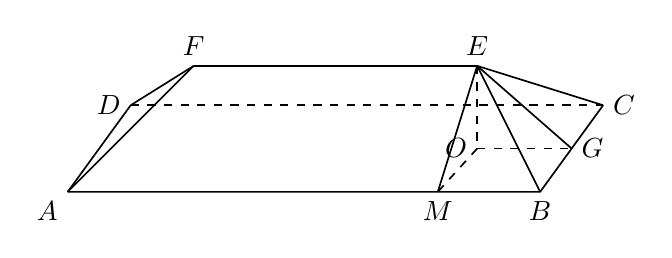
\begin{tikzpicture}[>=stealth,line width=0.6pt,font=\normalsize]
  \coordinate (A) at (0,0);
  \coordinate (B) at (6.0,0);
  \coordinate (C) at (6.8,1.1);
  \coordinate (D) at (0.8,1.1);
  \coordinate (F) at (1.6,1.6);
  \coordinate (E) at (5.2,1.6);

  % 外轮廓边
  \draw (A) -- (B) -- (C);
  \draw (A) -- (D);
  \draw (F) -- (E);
  \draw (F) -- (A);
  \draw (F) -- (D);
  \draw (E) -- (B);
  \draw (E) -- (C);
  \draw[dashed] (D) -- (C);

  % 辅助线 (从 E 点作垂线)
  \coordinate (O) at (5.2,0.55);
  \coordinate (M) at (4.7,0);
  \coordinate (G) at (6.4,0.55);

  \draw[dashed] (E) -- (O);
  \draw[dashed] (O) -- (M);
  \draw[dashed] (O) -- (G);
  \draw (E) -- (M);
  \draw (E) -- (G);

  % 标注
  \node[below left] at (A) {$A$};
  \node[below] at (B) {$B$};
  \node[right] at (C) {$C$};
  \node[left] at (D) {$D$};
  \node[above] at (F) {$F$};
  \node[above] at (E) {$E$};
  \node[left] at (O) {$O$};
  \node[below] at (M) {$M$};
  \node[right] at (G) {$G$};
\end{tikzpicture}
